This section provides an overview of the currently supported
equation sets. Equations will be decribed in integral form with
assumed Favre averaging. However, the laminar counterparts
are supported in the code base and are obtain in the user file
by ommitting a turbulence model specification.

\subsection{Conservation of Mass}
The continuity equation is always solved in the variable density form.

\begin{equation}
\int \frac{\partial \bar{\rho}} {\partial t}\, dV
+ \int \bar{\rho} \tilde{u}_i  n_i\, dS = 0
\end{equation}
Since Nalu uses equal-order interpolation (variables are collocated)
stabilization is required. The stabilization choice will be developed
in the pressure stabilization section.

Note that the use of a low speed compressible formulation requires that 
the fluid density be computed by an equation of state that uses the 
thermodynamic pressure. This thermodynamic pressure can either be computed
based on a global energy/mass balance or allowed to be spatially varying.
By modification of the continuity density time derivative to include 
the $\frac{\partial \rho}{\partial p}$ sensitivity,
an equation that admits acoustic pressure waves is realized.

\subsection{Conservation of Momentum}

The integral form of the Favre-filtered momentum equations used for
turbulent transport are
%
\begin{eqnarray}
   \int {{\partial \bar{\rho} \tilde{u}_i} \over {\partial t}} {\rm d}V
  +  \int \bar{\rho} \tilde{u}_i \tilde{u}_j n_j {\rm d}S 
  +  \int \bar{P} n_i {\rm d}S  &=& 
   \int \bar{\tau}_{ij} n_j {\rm d}S 
  + \int \tau_{u_i u_j} n_j {\rm d}S \nonumber \\ 
   &+& \int \left(\bar{\rho} - \rho_{\circ} \right) g_i {\rm d}V,
\label{fav-mom}
\end{eqnarray}
%
where the turbulent stress $\tau_{u_i u_j}$ is defined as
%
\begin{equation}
\tau_{u_i u_j} \equiv - \bar{\rho} ( \widetilde{u_i u_j} - 
     \tilde{u}_i \tilde{u}_j ).
\end{equation}
%
In a low Mach flow, as described in the low Mach theory section, 
the above pressure, $\bar P$ is the purturbation about the thermodynamic
pressure, $P^{th}$. In a low speed compressible flow, i.e., flows confinded to a closed
domain with energy or mass addition in which the continuity equation
has been modifed to accomodate accoustics, this pressure is interpreted at the
thermodynamic pressure itself.

For LES, $\tau_{u_i u_j}$ in Equation~\ref{fav-mom} represents the 
subgrid stress tensor.  The deviatoric part of the subgrid stress
tensor is defined as
%
\begin{eqnarray}
\tau_{u_i u_j}^D & \equiv & \tau_{u_i u_j} - \frac{1}{3} \tau_{u_k u_k}
                            \delta_{ij} \nonumber \\
    & = & \tau_{u_i u_j} + \frac{2}{3} \bar{\rho} q^2 \delta_{ij},
    \label{deviatoric-stress-les}
\end{eqnarray}
%
where the subgrid turbulent kinetic energy is defined as
$q^2 \equiv \frac{1}{2} (\widetilde{u_k u_k} - \tilde{u_k} \tilde{u_k} )$.
The deviatoric part of the subgrid stress tensor is then modeled similar
to RANS closures as,
%
\begin{equation}
\tau_{u_i u_j}^D = 2 \mu_t \left( \tilde{S}_{ij} - \frac{1}{3} \tilde{S}_{kk}
     \delta_{ij} \right).
\end{equation}
%
Substituting this into Equation~\ref{deviatoric-stress-les} yields the
modeled form of the full subgrid stress tensor
%
\begin{equation}
\tau_{u_i u_j} = 2 \mu_t \left( \tilde{S}_{ij} - \frac{1}{3} \tilde{S}_{kk}
     \delta_{ij} \right) - \frac{2}{3} \bar{\rho} q^2 \delta_{ij}.
\label{mod-stress-les}
\end{equation}

For low Mach-number flows, a vast majority of the turbulent kinetic energy
is contained at resolved scales.
For this reason, the subgrid turbulent kinetic energy $q^2$ will not be
directly treated and will instead be included in the pressure as an
additional normal stress.  The Favre-filtered momentum equations then become
%
\begin{eqnarray}
\lefteqn{ \int {{\partial \bar{\rho} \tilde{u}_i} \over {\partial t}}
     {\rm d}V + \int \bar{\rho} \tilde{u}_i \tilde{u}_j n_j {\rm d}S 
   + \int \left( \bar{P} + \frac{2}{3} \bar{\rho} q^2 \right) 
     n_i {\rm d}S = } \nonumber \\
   && \int 2 (\mu + \mu_t) \left( \tilde{S}_{ij} - \frac{1}{3}
      \tilde{S}_{kk} \delta_{ij} \right) n_j {\rm d}S
    + \int \left(\bar{\rho} - \rho_{\circ} \right) g_i {\rm d}V,
\label{mod-mom-les}
\end{eqnarray}
%
where LES closure models for the subgrid turbulent eddy viscosity
$\mu_t$ are either the constant coefficient Smagorinsky, WALE or the constant 
coefficient $k_{sgs}$ model (see the turbulence section).

\subsection{Filtered Mixture Fraction} \label{sec:filtered_Z}

The optional quantity used to identify the chemical state is the mixture 
fraction, $Z$.  While there are many 
different definitions of the mixture fraction that have subtle variations
that attempt to capture effects like differential diffusion, they can all 
be interpreted as a local mass fraction of the chemical elements that
originated in the fuel stream.  The mixture fraction is a
conserved scalar that varies between zero in the secondary stream and unity in the
primary stream and is transported in laminar flow by the equation,
%
\begin{equation}
\frac{\partial \rho Z}{\partial t}
  + \frac{ \partial \rho u_i Z }{ \partial x_i}
  = \frac{\partial}{\partial x_i} \left( \rho D \frac{\partial Z}{\partial x_i}
    \right),  \label{eqn:lam_Z}
\end{equation}
%
where $D$ is an effective molecular mass diffusivity.

Applying either temporal Favre filtering for RANS-based treatments or 
spatial Favre filtering for LES-based treatments yields


\begin{equation}
\int \frac{\partial \bar{\rho} \tilde{Z}}{\partial t} {\rm d}V
  + \int \bar{\rho} \tilde{u}_j \tilde{Z} n_j {\rm d}S
  = - \int \tau_{Zu_j} n_j {\rm d}S + \int \bar{\rho} D \frac{\partial \tilde{Z}}{\partial x_j} n_j {\rm d}S,  \label{eqn:turb_Z}
\end{equation}
%
where sub-filter correlations have been neglected in the molecular diffusive
flux vector and the turbulent diffusive flux vector is defined as
%
\begin{equation}
\tau_{Z u_j} \equiv \bar{\rho} \left( \widetilde{Z u_j} -
  \tilde{Z} \tilde{u}_j \right).
\end{equation}
%
This sub-filter correlation is modeled in
both RANS and LES closures with the gradient transport approximation
%
\begin{equation}
\tau_{Z u_j} \approx - \bar{\rho} D_t \frac{\partial Z}{\partial x_j},
\end{equation}
%
where $D_t$ is the turbulent mass diffusivity, modeled as $\bar{\rho} D_t =
\mu_t / \mathrm{Sc}_t$ where $\mu_t$ is the modeled turbulent viscosity
from momentum transport and $\mathrm{Sc}_t$ is the turbulent Schmidt number.
The molecular mass
diffusivity is then expressed similarly as $\bar{\rho} D = \mu / \mathrm{Sc}$
so that the final modeled form of the filtered mixture fraction transport
equation is
%
\begin{equation}
\frac{\partial \bar{\rho} \tilde{Z}}{\partial t}
  + \frac{ \partial \bar{\rho} \tilde{u}_i \tilde{Z} }{ \partial x_i}
  = \frac{\partial}{\partial x_i} 
    \left[ \left( \frac{\mu}{\mathrm{Sc}} + \frac{\mu_t}{\mathrm{Sc}_t} \right)
    \frac{\partial \tilde{Z}}{\partial x_i} \right].
\end{equation}
%
In integral form the mixture fraction transport equation is
%
\begin{equation}
\int \frac{\partial \bar{\rho} \tilde{Z}}{\partial t}\, dV
  + \int \bar{\rho} \tilde{u}_i \tilde{Z} n_i\, dS
  = \int \left( \frac{\mu}{\mathrm{Sc}} + \frac{\mu_t}{\mathrm{Sc}_t} \right)
    \frac{\partial \tilde{Z}}{\partial x_i} n_i\, dS.
\end{equation}

\subsection{Conservation of Energy}

The integral form of the Favre-filtered static enthalpy energy equation used for
turbulent transport is
%
\begin{eqnarray}
   \int {{\partial \bar{\rho} \tilde{h}} \over {\partial t}} {\rm d}V
  + \int \bar{\rho} \tilde{h} \tilde{u}_j n_j {\rm d}S 
  &=& - \int \bar{q}_j n_j {\rm d}S
  - \int \tau_{h u_j} n_j {\rm d}S 
  - \int {{\partial \bar{q}_i^r} \over {\partial x_i}} {\rm d}V \nonumber \\
  && + \int \left({{\partial \bar{P}} \over {\partial t}} + \tilde{u}_j {{\partial \bar{P}} \over {\partial x_j}}\right){\rm d}V
  + \int \overline{\tau_{ij} {{\partial u_i} \over {\partial x_j }}} {\rm d}V.
\label{fav-enth}
\end{eqnarray}
%

The above equation is derived by starting with the total internal energy
equation, subtracting the mechanical energy equation and enforcing the
variable density continuity equation. Note that the above equation includes
possible source terms due to thermal radiatitive transport, viscouss dissipation,
and pressure work.

The simple Fickian diffusion velocity approximation, Equation~\ref{diffvel1},
is assumed, so that the mean diffusive heat flux vector $\bar{q}_j$ is
%
\begin{eqnarray}
  \bar{q}_j = - \overline{ \left[ {\kappa \over {C_p}}
                       {{\partial h} \over {\partial x_j}}
                 -  {\mu \over {\rm Pr}} 
        \sum_{k=1}^K h_k {{\partial Y_k} \over {\partial x_j}} \right] }
     - \overline{ {\mu \over {\rm Sc}}
        \sum_{k=1}^K h_k {{\partial Y_k} \over {\partial x_j}} }.
\end{eqnarray}
%
If Sc = Pr, i.e., unity Lewis number (Le = 1), then the diffusive heat
flux vector simplifies to $\bar{q}_j = -\frac{\mu}{\mathrm{Pr}}
\frac{\partial \tilde{h}}{\partial x_j}$.  In the code base, the user
has the ability to either specify a laminar Prandtl number, which is
a constant, or provide a property evaluator for thermal conductivity. Inclusion
of a Prandtl number prevails and ensures that the thermal conductivity is computed
base on $\kappa = \frac{C_p \mu}{Pr}$. The viscous dissipation term is closed by
%
\begin{eqnarray}
\overline{\tau_{ij} {{\partial u_i} \over {\partial x_j }}}
  &=& \left(\left(\mu + \mu_t\right) \left( {{\partial \tilde{u}_i} 
      \over {\partial x_j}}
    + {{\partial \tilde{u}_j} \over {\partial x_i}} \right)
    - {2 \over 3} \left( \bar{\rho} \tilde{k} + 
      \mu_t{{\partial \tilde{u}_k} \over {\partial x_k}} \right)
      \delta_{ij} \right) {{\partial \tilde{u}_i} \over {\partial x_j}}
      \nonumber \\
  &=& \left[ 2 \mu \tilde{S}_{ij} 
    + 2 \mu_t \left( \tilde{S}_{ij} - \frac{1}{3} \tilde{S}_{kk}
      \delta_{ij} \right) - \frac{2}{3} \bar{\rho} \tilde{k}
      \delta_{ij} \right] \frac{\partial \tilde{u}_i}{\partial x_j}.
\end{eqnarray}
%
The turbulent diffusive flux vector $\tau_{h u_j}$ in Equation~\ref{fav-enth}
is defined as
%
\begin{equation}
\tau_{h u_j} \equiv \bar{\rho} \left( \widetilde{h u_j} - 
     \tilde{h} \tilde{u}_j \right).
\end{equation}
%
For RANS simulations, $\tau_{h u_j}$ represents the turbulent energy 
diffusive flux vector and is simplified to the form 
$\tau_{h u_j} = \overline{\rho h'' u_j''}$ by substitution of the 
Favre decomposition of each variable.  It is then modeled by
%
\begin{equation}
\tau_{h u_j} = \overline{\rho h'' u_j''}
   = - \frac{\mu_t}{\mathrm{Pr}_t} \frac{\partial \tilde{h}}{\partial x_j},
\end{equation}
%
where $\mathrm{Pr}_t$ is the turbulent Prandtl number and $\mu_t$ is 
the modeled turbulent eddy viscosity from momentum closure.  For LES, 
$\tau_{h u_j}$ represents
the subgrid turbulent energy diffusive flux vector, and is modeled in the
same way as
%
\begin{equation}
\tau_{h u_j} = - \frac{\mu_t}{\mathrm{Pr}_t} \frac{\partial 
     \tilde{h}}{\partial x_j},
\end{equation}
%
where $\mathrm{Pr}_t$ is the subgrid turbulent Prandtl number and $\mu_t$
is the modeled subgrid turbulent eddy viscosity from momentum closure.

The resulting filtered and modeled turbulent energy equation for both RANS
and LES is given by,
%
\begin{eqnarray}
\int {{\partial \bar{\rho} \tilde{h}} \over {\partial t}} {\rm d}V
   + \int \bar{\rho} \tilde{h} \tilde{u}_j n_j {\rm d}S 
 &=& \int \left( {\mu \over {\rm Pr}} + {{\mu_t} \over {{\rm Pr}_t}} \right) 
     {{\partial \tilde{h}} \over {\partial x_j}}  n_j {\rm d}S 
   - \int {{\partial \bar{q}_i^r} \over {\partial x_i}} {\rm d}V \nonumber \\
 &+& \int \left({{\partial \bar{P}} \over {\partial t}} + \tilde{u}_j 
     {{\partial \bar{P}} \over {\partial x_j}}\right){\rm d}V
   + \int \overline{\tau_{ij} {{\partial u_j} \over {\partial x_j }}} {\rm d}V.
\label{mod-enth}
\end{eqnarray}
%
The turbulent Prandtl number must have the same value as
the turbulent Schmidt number for species transport to maintain unity Lewis
number.

\subsubsection{Review of Prandtl, Schmidt and Unity Lewis Number}

For situations where a single diffusion coefficient is applicable (e.g., a binary gas system) the Lewis number is defined as:

\begin{eqnarray}
{\rm Le} = {{\rm Sc} \over {\rm Pr}} = {{\alpha} \over {D}}. 
\label{lewisNumber}
\end{eqnarray}
%
If the diffusion rates of energy and mass are equal, 

\begin{eqnarray}
{\rm Sc = Pr \ and \ Le = 1}. 
\label{lewisNumberUnity}
\end{eqnarray}
%
For completeness, the thermal diffusivity, Prandtl and Schmidt number are defined by,

\begin{eqnarray}
\alpha = {{\kappa} \over {\rho c_p}},
\label{thermalDiff}
\end{eqnarray}

\begin{eqnarray}
{\rm Pr} = {{c_p \mu } \over {\kappa}} = {{\mu} \over {\rho \alpha}},
\label{prandtl}
\end{eqnarray}
%
and
\begin{eqnarray}
{\rm Sc} = {{\mu } \over {\rho D}}, 
\label{schmidt}
\end{eqnarray}
where $c_p$ is the specific heat, $\kappa$, is the thermal conductivity and
$\alpha$ is the thermal diffusivity.


\subsection{Thermal Heat Conduction}

For non-isothermal object response that may occur in conjugate heat transfer
applications, a simple single material heat conduction equation is supported.
%
\begin{equation}
  \int \rho C_p \frac{\partial T} {\partial t} {\rm d}V
  + \int q_j n_j {\rm d}S = \int S {\rm d}V.
\label{thermalHeatEquation}
\end{equation}
where $q_j$ is again the energy flux vector, however, now in the following 
temperature form:

\begin{equation}
 q_j = -\kappa \frac{\partial T}{\partial x_j}.
\end{equation}

\subsection{Conservation of Species}

The integral form of the Favre-filtered species equation used for
turbulent transport is
%
\begin{equation}
  \int {{\partial \bar{\rho} \tilde{Y}_k} \over {\partial t}} {\rm d}V
  + \int \bar{\rho} \tilde{Y}_k \tilde{u}_j n_j {\rm d}S = 
  - \int \tau_{Y_k u_j} n_j {\rm d}S
  - \int \overline{\rho Y_k \hat{u}_{j,k}} n_j {\rm d}S + 
   \int \overline{\dot{\omega}_k} {\rm d}V,
\label{fav-species}
\end{equation}
%
where the form of diffusion velocities (see Equation~\ref{diffvel1}) assumes 
the Fickian approximation with a constant value of diffusion velocity 
for consistency with the turbulent form of the energy equation, 
Equation~\ref{fav-enth}. The simplest form is Fickian diffusion with the same  
value of mass diffusivity for all species,  
%
\begin{equation}
  \hat{u}_{j,k}= - D {1 \over {Y_k}} 
                   {{\partial Y_k} \over {\partial x_j}} .
  \label{diffvel1}
\end{equation}
%
The turbulent diffusive flux vector $\tau_{Y_k u_j}$ is defined as
%
\begin{equation}
\tau_{Y_k u_j} \equiv \bar{\rho} \left( \widetilde{Y_k u_j} - 
     \tilde{Y_k} \tilde{u}_j \right).
\end{equation}
%
For RANS simulations, $\tau_{Y_k u_j}$ represents the turbulent species 
diffusive flux vector and is simplified to the form 
$\tau_{Y_k u_j} = \overline{\rho Y_k'' u_j''}$ by substitution of the 
Favre decomposition of each variable.  It is then modeled as
%
\begin{equation}
\tau_{Y_k u_j} = \overline{\rho Y_k'' u_j''}
    = - \frac{\mu_t}{\mathrm{Sc}_t} \frac{\partial \tilde{Y}_k}{\partial x_j}, 
\end{equation}
%
where $\mathrm{Sc}_t$ is the turbulent Schmidt number for all species
and $\mu_t$ is the modeled turbulent eddy viscosity from momentum closure.
For LES, $\tau_{Y_k u_j}$ represents the subgrid turbulent species diffusive 
flux vector, and is modeled identically as
%
\begin{equation}
\tau_{Y_k u_j} = - \frac{\mu_t}{\mathrm{Sc}_t} \frac{\partial 
     \tilde{Y}_k}{\partial x_j}, 
\end{equation}
%
where $\mathrm{Sc}_t$ is the subgrid turbulent Schmidt number for all
species and $\mu_t$ is the subgrid modeled turbulent eddy viscosity from
momentum closure.

The Favre-filtered and modeled turbulent species transport equation
for both RANS and LES then becomes
%
\begin{equation}
  \int {{\partial \bar{\rho} \tilde{Y}_k} \over {\partial t}} {\rm d}V
  + \int \bar{\rho} \tilde{Y}_k \tilde{u}_j n_j {\rm d}S = 
   \int \left( {\mu \over {\rm Sc}} 
              + {{\mu_t} \over {{\rm Sc}_t}}  \right)
          {{\partial \tilde{Y}_k} \over
           {\partial x_j}} n_j {\rm d}S + 
   \int \overline{\dot{\omega}}_k {\rm d}V .
\label{mod-species}
\end{equation}

If transporting both energy and species equations, the laminar Prandtl 
number must be equal to the laminar Schmidt number and the turbulent 
Prandtl number must be equal to the turbulent Schmidt number to maintain
unity Lewis number.  Although there is a species conservation equation 
for each species in a mixture of  $n$ species, only $n-1$ species equations
need to be solved since the mass fractions sum to unity and
%
\begin{equation}
  \tilde{Y}_n = 1 - \sum_{j \ne n}^{n} \tilde{Y}_j .
\end{equation}

Finally, the reaction rate source term is expected to be added based on an
operator split approach wherebye the set of ODEs are integrated over the full
time step. The chemical kinetic source terms can be sub-integrated within
a time step using a stiff ODE integrator package. 

The following system of ODEs are numerically integrated over a time 
step $\Delta t$ for a fixed temperature and pressure starting from 
the initial values of gas phase mass fraction and density,
\begin{equation}
  \dot{Y}_k = {{\dot{\omega}_k \left( Y_k \right) } \over \rho} \ .
\end{equation}
The sources for the sub-integration are computed with the composition and density at the 
new time level which are used to approximate a mean production rate for the time step
\begin{equation}
  \dot{\omega}_k \approx {{\rho^{\ast} Y^{\ast}_k - \rho Y_k}
                           \over {\Delta t}} \ .
\end{equation}

\subsection{Subgrid-Scale Kinetic Energy One-Equation LES Model}

The subgrid scale kinetic energy one-equation turbulence model, or 
$k^{sgs}$ model,~\cite{Davidson:1997}, represents a simple LES closure model.  The transport 
equation for subgrid turbulent kinetic energy is given by
%
\begin{equation}
  \int {{\partial \bar{\rho}{k^\mathrm{sgs}}} \over {\partial t}} {\rm d}V
  + \int \bar{\rho}{k^\mathrm{sgs}} \tilde{u}_j n_j {\rm d}S = 
    \int {{\mu_t} \over {\sigma_k}} 
          {{\partial {k^\mathrm{sgs}}} \over
           {\partial x_j}} n_j {\rm d}S + 
   \int \left(P_k^\mathrm{sgs} - D_k^\mathrm{sgs}\right) {\rm d}V.
\label{ksgs}
\end{equation}
%
The production of subgrid turbulent kinetic energy, $P_k^\mathrm{sgs}$, is 
modeled by,
\begin{equation}
   P_k \equiv  -\overline{\rho u_i'' u_j''}
      {{\partial \tilde{u}_i} \over {\partial x_j}},
\label{mod-prod}     
\end{equation}
while the dissipation of turbulent kinetic energy, $D_k^\mathrm{sgs}$, is given by
%
\begin{equation}
D_k^\mathrm{sgs} = C_{\epsilon} { { {k^\mathrm{sgs}}^{{3}\over {2}} } 
     \over { \Delta} },
\end{equation}
%
where the grid filter length, $\Delta$, is given in terms of the grid cell
volume by
%
\begin{equation}
\Delta = V^{{1}\over{3}}.
\end{equation}

The subgrid turbulent eddy viscosity is then provided by 
%
\begin{equation}
\mu_t = C_{\mu_{\epsilon}} \Delta {k^\mathrm{sgs}}^{{1} \over {2}},
\end{equation}
%
where the values of $C_{\epsilon}$ and $C_{\mu_{\epsilon}}$ are 
0.845 and 0.0856, respectively.

\subsection{Shear Stress Transport (SST) RANS Model Suite} \label{sec:sst}
Although Nalu is primarily expected to be a LES simulation tool, RANS modeling is supported
through the activation of the SST equation set.

It has been observed that standard 1998 $k-\omega$ models display a strong sensitivity 
to the free stream value of $\omega$ (see Mentor,~\cite{Mentor:2003}).  To remedy, this, an 
alternative set of transport equations have been used that are based on smoothly 
blending the $k-\omega$ model near a wall with $k-\epsilon$ away from the wall.  
Because of the relationship between $\omega$ and $\epsilon$, the transport equations 
for turbulent kinetic energy and dissipation can be transformed into equations 
involving $k$ and $\omega$.  Aside from constants, the transport equation for 
$k$ is unchanged.  However, an additional cross-diffusion term is present in 
the $\omega$ equation.  Blending is introduced by using smoothing which is a 
function of the distance from the wall, $F(y)$.  The transport equations for the Mentor 2003 model
 are then

\begin{eqnarray}
\int{\partial \bar{\rho} k \over \partial t}\text{d}V + \int \bar{\rho} k\tilde{u}_{j} n_{j} \text{d} S = \int {(\mu + \hat \sigma_k \mu_{t})} {\partial k \over \partial x_{j}} n_{j} + \int \left(P_{k}^{\omega} - \beta^* \bar{\rho} k \omega\right) \text{d} V,
\end{eqnarray}

\begin{eqnarray}
\int {\partial \bar{\rho} \omega \over \partial t}\text{d} V + \int \bar{\rho} \omega \tilde{u}_{j} n_{j} \text{d}S &=& 
\int  {(\mu + \hat\sigma_{\omega} \mu_{t})} {\partial \omega \over \partial x_{j}} n_{j}
+ \int  {2(1-F) \frac{\bar{\rho}\sigma_{\omega2}} {\omega} {\partial k \over \partial x_j} {\partial \omega \over \partial x_j} } \text{d}V \nonumber \\ 
&+&  \int \left(\frac{\hat\gamma}{\nu_t} P_{k}^{\omega} - \hat \beta \bar{\rho} \omega^{2}\right) \text{d}V.
\end{eqnarray}
%
The model coefficients, $\hat\sigma_k$, $\hat\sigma_{\omega}$, $\hat\gamma$ and $\hat\beta$ must also be blended, which is represented by
\begin{equation}
\hat \phi = F\phi_1+ (1-F)\phi_2.
\end{equation}
where $\sigma_{k1} = 0.85$, $\sigma_{k2} = 1.0$,  $\sigma_{\omega1} = 0.5$, $\sigma_{\omega2} = 0.856$, $\gamma_1 = \frac{5}{9}$, $\gamma_2 = 0.44$,
$\beta_1 = 0.075$ and $\beta_2 = 0.0828$.  
%
The blending function is given by
\begin{equation}
F = \tanh(arg_{1}^{4}),
\end{equation}
where
\begin{equation}
arg_{1} = \min \left( \max \left( {\sqrt{k} \over \beta^* \omega y}, {500 \mu \over \bar{\rho} y^{2} \omega}\right), {4 \bar{\rho} \sigma_{\omega2} k \over CD_{k\omega} y^{2}} \right).
\end{equation}
The final parameter is
\begin{equation}
CD_{k\omega} = \max \left( 2 \bar{\rho} \sigma_{\omega2} \frac{1}{\omega} {\partial k \over \partial x_{j}} {\partial \omega \over \partial x_{j}}, 10^{-10} \right).
\end{equation}

An important component of the SST model is the different expression used for the turbulent viscosity,
\begin{equation}
\mu_{t} = \frac {a_1 \bar{\rho} k} {\max\left( a_1 \omega, S F_2 \right) },
\end{equation}
where $F_2$ is another blending function given by
\begin{equation}
F_2 = \tanh(arg_{2}^{2}).
\end{equation}
The final parameter is
\begin{equation}
arg_{2} = \max\left({2 \sqrt{k} \over \beta^* \omega y}, {500 \mu \over \bar{\rho} \omega y^{2}} \right).
\end{equation}

\subsubsection{Direct Eddy Simulation (DES) Formulation}
The DES technique is also supported in the code base when the SST model is activated. 
This model seeks to formally relax the RANS-based approach and allows for a theoretical
basis to allow for transient flows. The method follows the method of Temporally
Filtered NS formulation as decribed by Tieszen,~\cite{Tieszen:2005}.

The SST DES model simply changes the turbulent kinetic energy equation to include
a new minimum scale that manipulates the dissipation term.

\begin{equation}
D_k = \frac{\rho k^{3/2}} {l_{DES}},
\end{equation}
where $l_{DES}$ is the min($l_{SST}, c_{DES}l_{DES}$). The constants are given by, 
$l_{SST}=\frac{k^{1/2}}{\beta^* \omega}$ and $c_{DES}$ represents a blended set of 
DES constants: $c_{{DES}_1} = 0.78$ and  $c_{{DES}_2} = 0.61$. The length scale, $l_{DES}$
is the maximum edge length scale touching a given node. 

\subsection{Solid Stress}

A fully implicit CVFEM (only) linear elastic equation is supported in the code base. 
This equation is either used for true solid stress prediction or for smoothing the
mesh due to boundary mesh motion (either through fluid structure interaction (FSI) or
prescribed mesh motion).

Consider the displacement for component i, $u_i$ equation set,

\begin{equation}
 \rho \frac{\partial^2 u_i} {{\partial t}^2} - \frac{\partial \sigma_{ij}}{\partial x_j} = F_i,
\label{linearElastic}
\end{equation}
where the Cauchy stress tensor, $\sigma_{ij}$ assuming Hooke's law is given by,

\begin{equation}
 \sigma_{ij} = \mu \left ( \frac{\partial u_i}{\partial x_j} +  \frac{\partial u_j}{\partial x_i} \right)
 + \lambda \frac{\partial u_k}{\partial x_k} \delta_{ij}.
\label{stress}
\end{equation}

Above, the so-called Lame coefficients, Lame's first parameter, $\lambda$ (also known 
as the Lame modulus) and Lame's second parameter, $\mu$ (also known as the shear modulus) 
are provided as functions of the Young's modulus, $E$, and Poisson's ratio, $\nu$; 
here shown in the context of a isotropic elastic material,

\begin{equation}
 \mu = \frac{E}{2\left(1+\nu\right)},
\label{lame_mu}
\end{equation}
and
\begin{equation}
 \lambda = \frac{E \nu}{\left(1+\nu\right) \left(1-2 \nu \right)}.
\label{lame_lambda}
\end{equation}

Note that the above notation of $u_i$ to represent displacement is with respect to
the classic definition of current and model coordinates,

\begin{equation}
 x_i = X_i + u_i
\label{displacement}
\end{equation}
where $x_i$ is the position, relative to the fixed, or previous position, $X_i$.

The above equations are solved for mesh displacements, $u_i$. The supplemental
relationship for solid velocity, $v_i$ is given by,

\begin{equation}
 v_i = \frac{\partial u_i}{\partial t}.
\label{velocity}
\end{equation}
Numerically, the velocity might be obtained by a backward Euler or BDF2 scheme,
\begin{equation}
 v_i = \frac{\gamma_1 u^{n+1}_i + \gamma_2 u^n_i + \gamma_3 u^{n-1}_i}{\Delta t}
\label{mesh_velocity+numerical}
\end{equation}

\subsection{Moving Mesh}
The code base supports three notions of moving mesh: 1) linear elastic equation system
that computes the stress of a solid 2) solid body rotation mesh motion and 3) mesh 
mesh deformation via an external source.

The linear elastic equation system is activated via the standard equation system approach.
Properties for the solid are specified in the material block. Mesh motion is prescribed by 
the input file via the ''$mesh \textunderscore motion$'' block. Here, it is assumed that the mesh motion 
is solid rotation. For fluid/structure interaction
(FSI) a mesh smoothing scheme is used to propagate the surface mesh displacement
obtained by the solids solve. Simple mesh smoothing is obtained via a linear elastic 
solve in which the so-called Lame constants are proportional to the inverse of the
dual volume. This allows for boundary layer mesh locations to be stiff while free 
stream mesh elements to be soft. 

Additional mesh motion terms are required for the Eulerian fluid mechanics solve.
Using the geometric conservative law the time and advection source term for a general
scalar $\phi$ can be written as:

\begin{equation}
   \int \frac {\rho \phi } {\partial t}\, dV + \int \rho \phi \left ( u_j - v_j \right) n_j\, dS 
   + \int \rho \phi \frac{\partial v_k}{\partial x_j}\, dV,
\label{gcl}
\end{equation}
where  $u_j$ is the fluid velocity and $v_j$ is the mesh velocity. Mesh velocities and the 
mesh velocity spatial derivatives are provided by the mesh smoothing solve. Activating the external
mesh deformation or mesh motion block will result in the velocity relative to mesh calculation
in the advection terms. The  line command for source term, ``$gcl$'' must be activated for each equation for 
the volume integral to be included in the set of PDE solves.
Finally, transfers are expected between the physics. For example, the solids solve is to provide mesh
displacements to the mesh smoothing realm. The mesh smoothing procedure provides the boundary velocity,
mesh velocity and projected nodal gradients of the mesh velocity to the fluids realm. Finally, the fluids
solve is to provide the surface force at the desired solids surface. Currently, the pressure is transfered
from the fluids realm to the solids realm. The ideal view of FSI is to solve the solids pde at the half 
time step. As such, in time, the $P^{n+\frac{1}{2}}$ is expected. The ``$fsi \textunderscore interface$'' 
input line command attribute is expected to be set at these unique surfaces. More advanced FSI coupling 
techniques are under development by a current academic partner.

\subsection{Radiative Transport Equation}
The spatial variation of the radiative intensity corresponding to 
a given direction and at a given wavelength within a radiatively 
participating material, $I(s)$, is governed by the Boltzmann transport 
equation.  In general, the Boltzmann equation represents a balance 
between absorption, emission, out-scattering, and in-scattering of 
radiation at a point.  For combustion applications, however, the 
steady form of the Boltzmann equation is appropriate since the 
transient term only becomes important on nanosecond time scales 
which is orders of magnitude shorter than the fastest chemical.

Experimental data shows that the radiative properties for 
heavily sooting, fuel-rich hydrocarbon diffusion flames 
($10^{-4}$\% to $10^{-6}$\% soot by volume) are dominated by 
the soot phase and to a lesser extent by the gas phase. Since 
soot emits and absorbs radiation in a relatively constant 
spectrum, it is common to ignore wavelength effects when modeling 
radiative transport in these environments.  Additionally, scattering 
from soot particles commonly generated by hydrocarbon flames is 
several orders of magnitude smaller that the absorption effect 
and may be neglected.  Moreover, the phase function is rarely known. However,
for situations in which the phase function can be approximated by the iso-tropic scattering
assumption, i.e., an intensity for direction $k$ has equal probability to be scattered
in any direction $l$, the appropriate form of the Botzmann radiative transport is
%
\begin{equation}
   s_i {{\partial} \over {\partial x_i}} I\left(s\right)
   + \left(\mu_a + \mu_s \right) I\left(s\right) = {{\mu_a \sigma T^4} \over {\pi}} + \frac{\mu_s}{4\pi}G,
\label{lam-scalar-flux}
\end{equation}
%
where $\mu_a$ is the absorption coeffiecient, $\mu_s$ is the scattering
coefficeint, $I(s)$ is the intensity 
along the direction $s_i$, $T$ is the temperature and the scalar flux is $G$. 
The black body radiation, $I_b$, is defined by $\frac{\sigma T^4}{\pi}$.
Note that for situations in which the scattering coefficient is zero, the RTE
reduces to a set of liniear, decoupled equations for each intensity to be solved.  

The flux divergence may be written 
as a difference between the radiative emission and mean incident 
radiation at a point,
%
\begin{equation}
   {{\partial q_i^r} \over {\partial x_i}} =
    \mu_a \left[ 4 \sigma T^4 - G \right] ,
\label{div-qrad}
\end{equation}
%
where $G$ is again the scalar flux. The flux divergence term is the same regardless
of whether or not scattering is active. The quantity, $G/4\pi$, is often 
referred to as the mean incident intensity. Note that when the scattering 
coefficient is non-zero, the RTE is coupled over all intensity directions by
the scalar flux relationship.

The scalar flux and radiative flux vector represent angular 
moments of the directional radiative intensity at a 
point,
%
\begin{equation}
   G = \int_{0}^{2\pi}\!\int_{0}^{\pi}\! I\left(s\right)
        \sin \theta_{zn} d \theta_{zn} d \theta_{az} ,
\end{equation}
%
\begin{equation}
   q^{r}_{i} = \int_{0}^{2\pi}\!\int_{0}^{\pi}\! I\left(s\right)
        s_i \sin \theta_{zn} d \theta_{zn} d \theta_{az} ,
\end{equation}
%
where $\theta_{zn}$ and $\theta_{az}$ are the zenith and azimuthal 
angles respectively as shown in Figure~\ref{ord-dir}.

\begin{figure}[ht]
\centerline{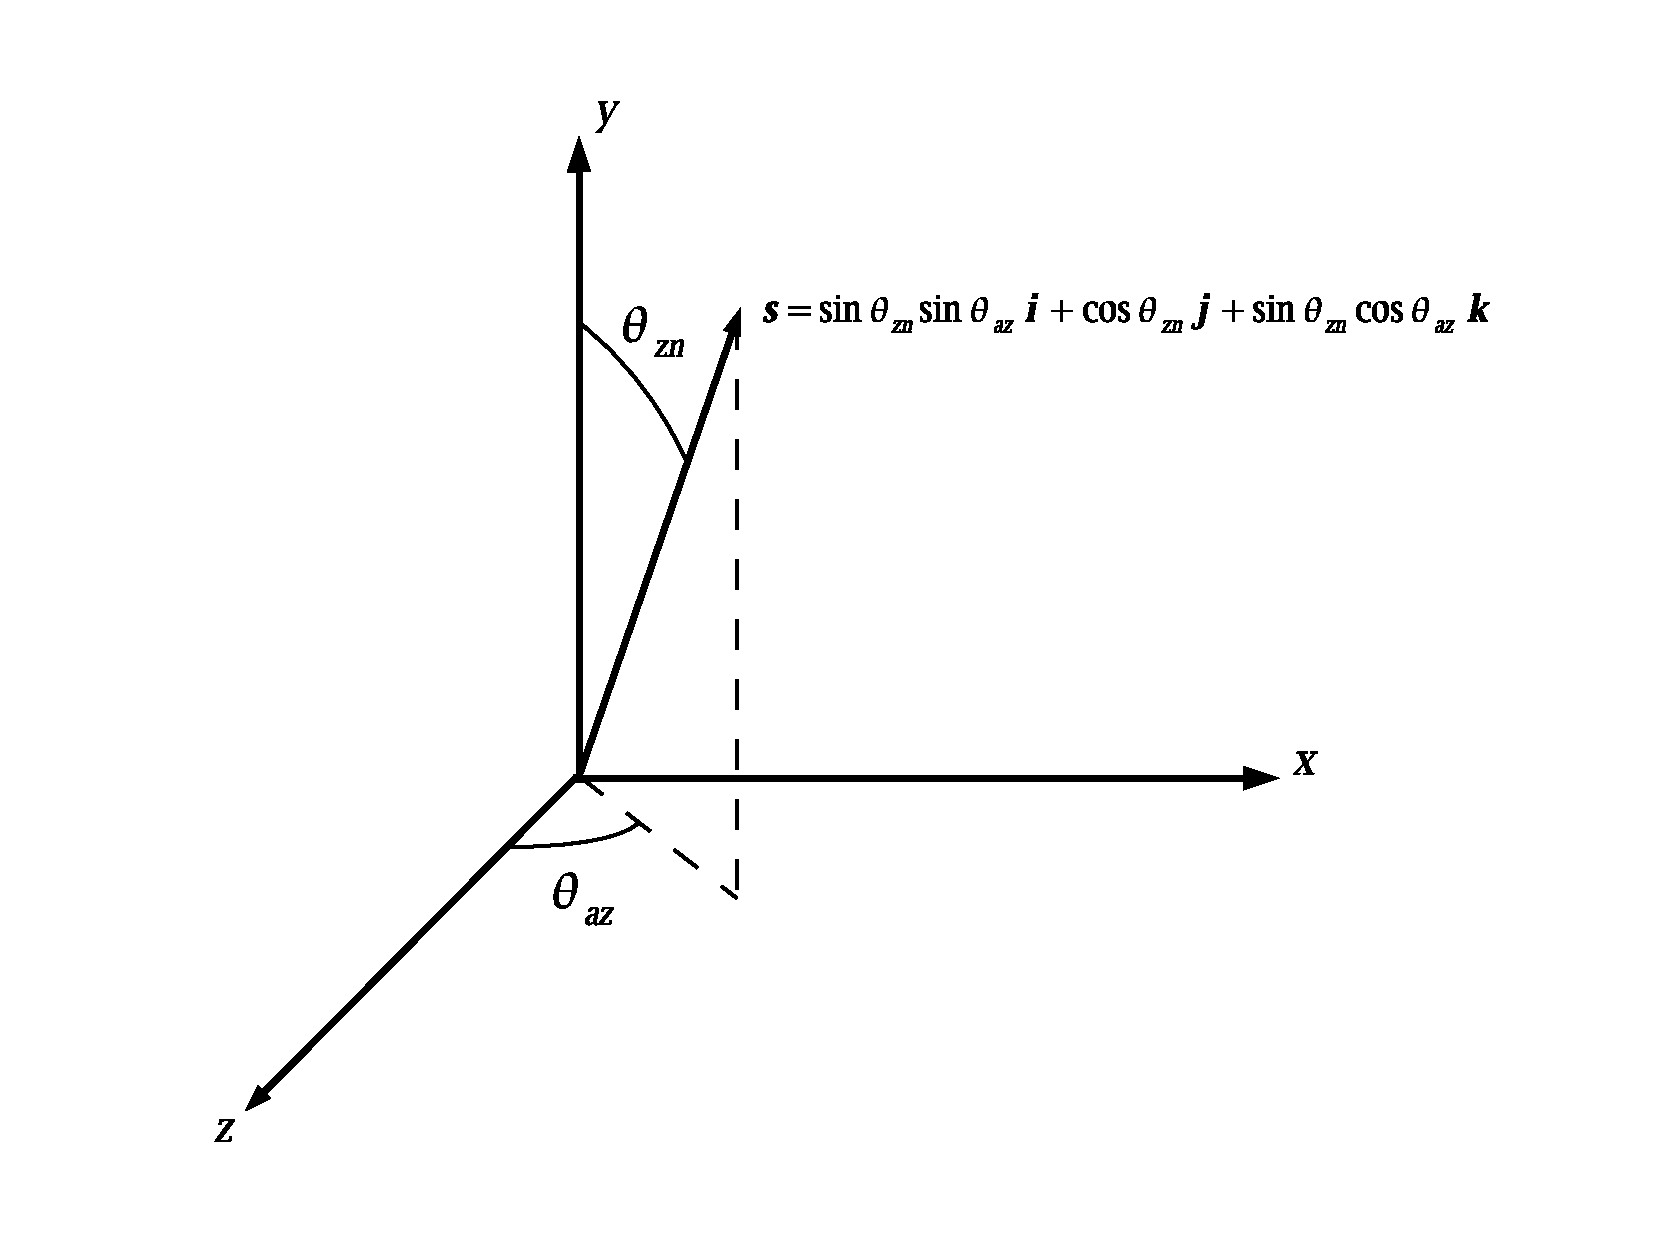
\includegraphics[width=3.0in]{images/ordinate.pdf}}
\vspace{0.1in}
\caption{Ordinate Direction Definition, \newline
         ${\bf s} = \sin \theta_{zn} \sin \theta_{az} {\bf i}
            + \cos \theta_{zn} {\bf j} 
            + \sin \theta_{zn} \cos \theta_{az} {\bf k}$}
\label{ord-dir}
\end{figure}


The radiation intensity must be defined at all portions 
of the boundary along which $s_i n_i < 0$, where $n_i$ is the 
outward directed 
unit normal vector at the surface.  The intensity is applied as a 
weak flux boundary condition which is determined from the surface 
properties and temperature.  The diffuse surface assumption 
provides reasonable accuracy for many engineering combustion 
applications.  The intensity leaving a diffuse surface in all 
directions is given by
%
\begin{equation}
  I\left(s\right) = {1 \over \pi} \left[ \tau \sigma T_\infty^4 
                  + \epsilon \sigma T_w^4
                  + \left(1 - \epsilon - \tau \right) K \right] ,
\label{intBc}
\end{equation}
%
where $\epsilon$ is the total normal emissivity of the 
surface, $\tau$ is the transmissivity of the surface, $T_w$ is the 
temperature of the boundary, $T_\infty$ is the environmental 
temperature and  $H$ is the incident radiation, or irradiation (incoming radiative flux). 
Recall that the relationship given by Kirchoff's 
Law that relates emissivity, transmissivity and reflectivity, $\rho$, is
%
\begin{equation}
  \rho + \tau + \epsilon = 1.
\end{equation}
%
where it is implied that $\alpha = \epsilon$.
